\chapter{The First Analog Prototype: First Resets and Leakage Measurements}~\label{chap:saq}

In this chapter we present the first implementation of the Q-Pix front-end design using off-the-shelf electronics.

This section describes the first prototype based on the Q-Pix readout: The Simplified Analog Q-Pix (SAQ).
First we discuss the design goals of the prototype and highlight the basic building blocks of any Q-Pix based prototype.
We present these results as a demonstration Q-Pix timestamp procedure to perform measurements.
Next, We describe the prototype status as well as lessons learned in characterizing noise and performing calibrations.

In the final part of this section we briefly describe the future goals of this prototype, including the calibration of the detector response with Gas Electron Multipliers (GEMs)~\citep{SAULI20162}.
We emphasize that at the time of the writing of this thesis the acquisition and analysis of data from this experiment are incomplete.
Nevertheless, the lessons learned so far, particularly in calibration, are useful to explore the abilities of the Q-Pix readout.
The final results of SAQ are just beyond the scope of this work, but we provide SAQ's details here as a means of introducing the front-end of Q-Pix as well as highlighting my personal contributions to Q-Pix's overall development.

The entire data acquisition (DAQ) chain used for both SAQ experimental setups are my sole independent work.
My contributions include the the development and deployement firmware on the Zybo-Z7 FPGA, as well as the embedded software code on the integrated SoC processing system.
I developed the the Python3 software which handles packet communication as well as the GUI for data collection.
I also developed the data storage trees, which are the original containers for all data used in the analysis. 
Additionally, I wrote analysis scripts used for the work done at the SAQ site at the University of Texas at Arlington.

\section{Simplified Analog Q-Pix: System Design}

The Simplified Analog Q-Pix (SAQ) experiment aims to demonstrate the first physics measurement using the analog front-end of a Q-Pix based readout.
The desired measurement is the transverse diffusion of electron in Argon gas~(Equation~\ref{eq:diffusion}).
In the simplest case, the diffusion of electrons within a TPC is described by:
\begin{equation}~\label{eq:diffusion}
 \sigma^{2}_{T} = 2D_{trans}L
\end{equation}
Where L is the drift length of the electrons, $D_{trans}$ is the (field dependent) diffusion coeffecient, and $\sigma^{2}_(T)$ is the transverse diffusion standard deviation.
Q-Pix could perform a measurement of $\sigma_{T}$ in Equation~\ref{eq:diffusion} by either collecting a different amount of charge or current at different radii from the center.

A diffusion measurement is a natural starting point to verify a charge accumulation readout such as Q-Pix.
One difference between SAQ and a "normal" Q-Pix readout is that instead of separated pixels SAQ uses a series of 16 concentric rings at the collection plane.
Although separated pixels may be used, the effect of transverse diffusion is radially symmetric about the collection plane; the use of circular 'pixels' reduces the amount digitization channels.

SAQ has built two different TPCs: one at the University of Texas at Arlington (UTA) and the other at Wellesley College.
The experimental setup at UTA is shown in Figure~\ref{fig:saq_setup_flatten}, and the setup at Wellesley is shown in Figure~\ref{fig:wellesley_tpc}.
Both TPCs shown are circular TPCs with a drift length of $\approx 10~\unit{cm}$.

The experimental setups at both UTA and Wellesley are nearly identical except for the placement of the readout electronics.
The SAQ readout board for UTA is placed on the outside of the TPC, whereas it is placed within a P10 argon gas, but not within the field cage of the TPC.
The detection within the TPC at UTA is an ultra pure (99.99\%) argon gas.

\begin{figure}[]
\centering
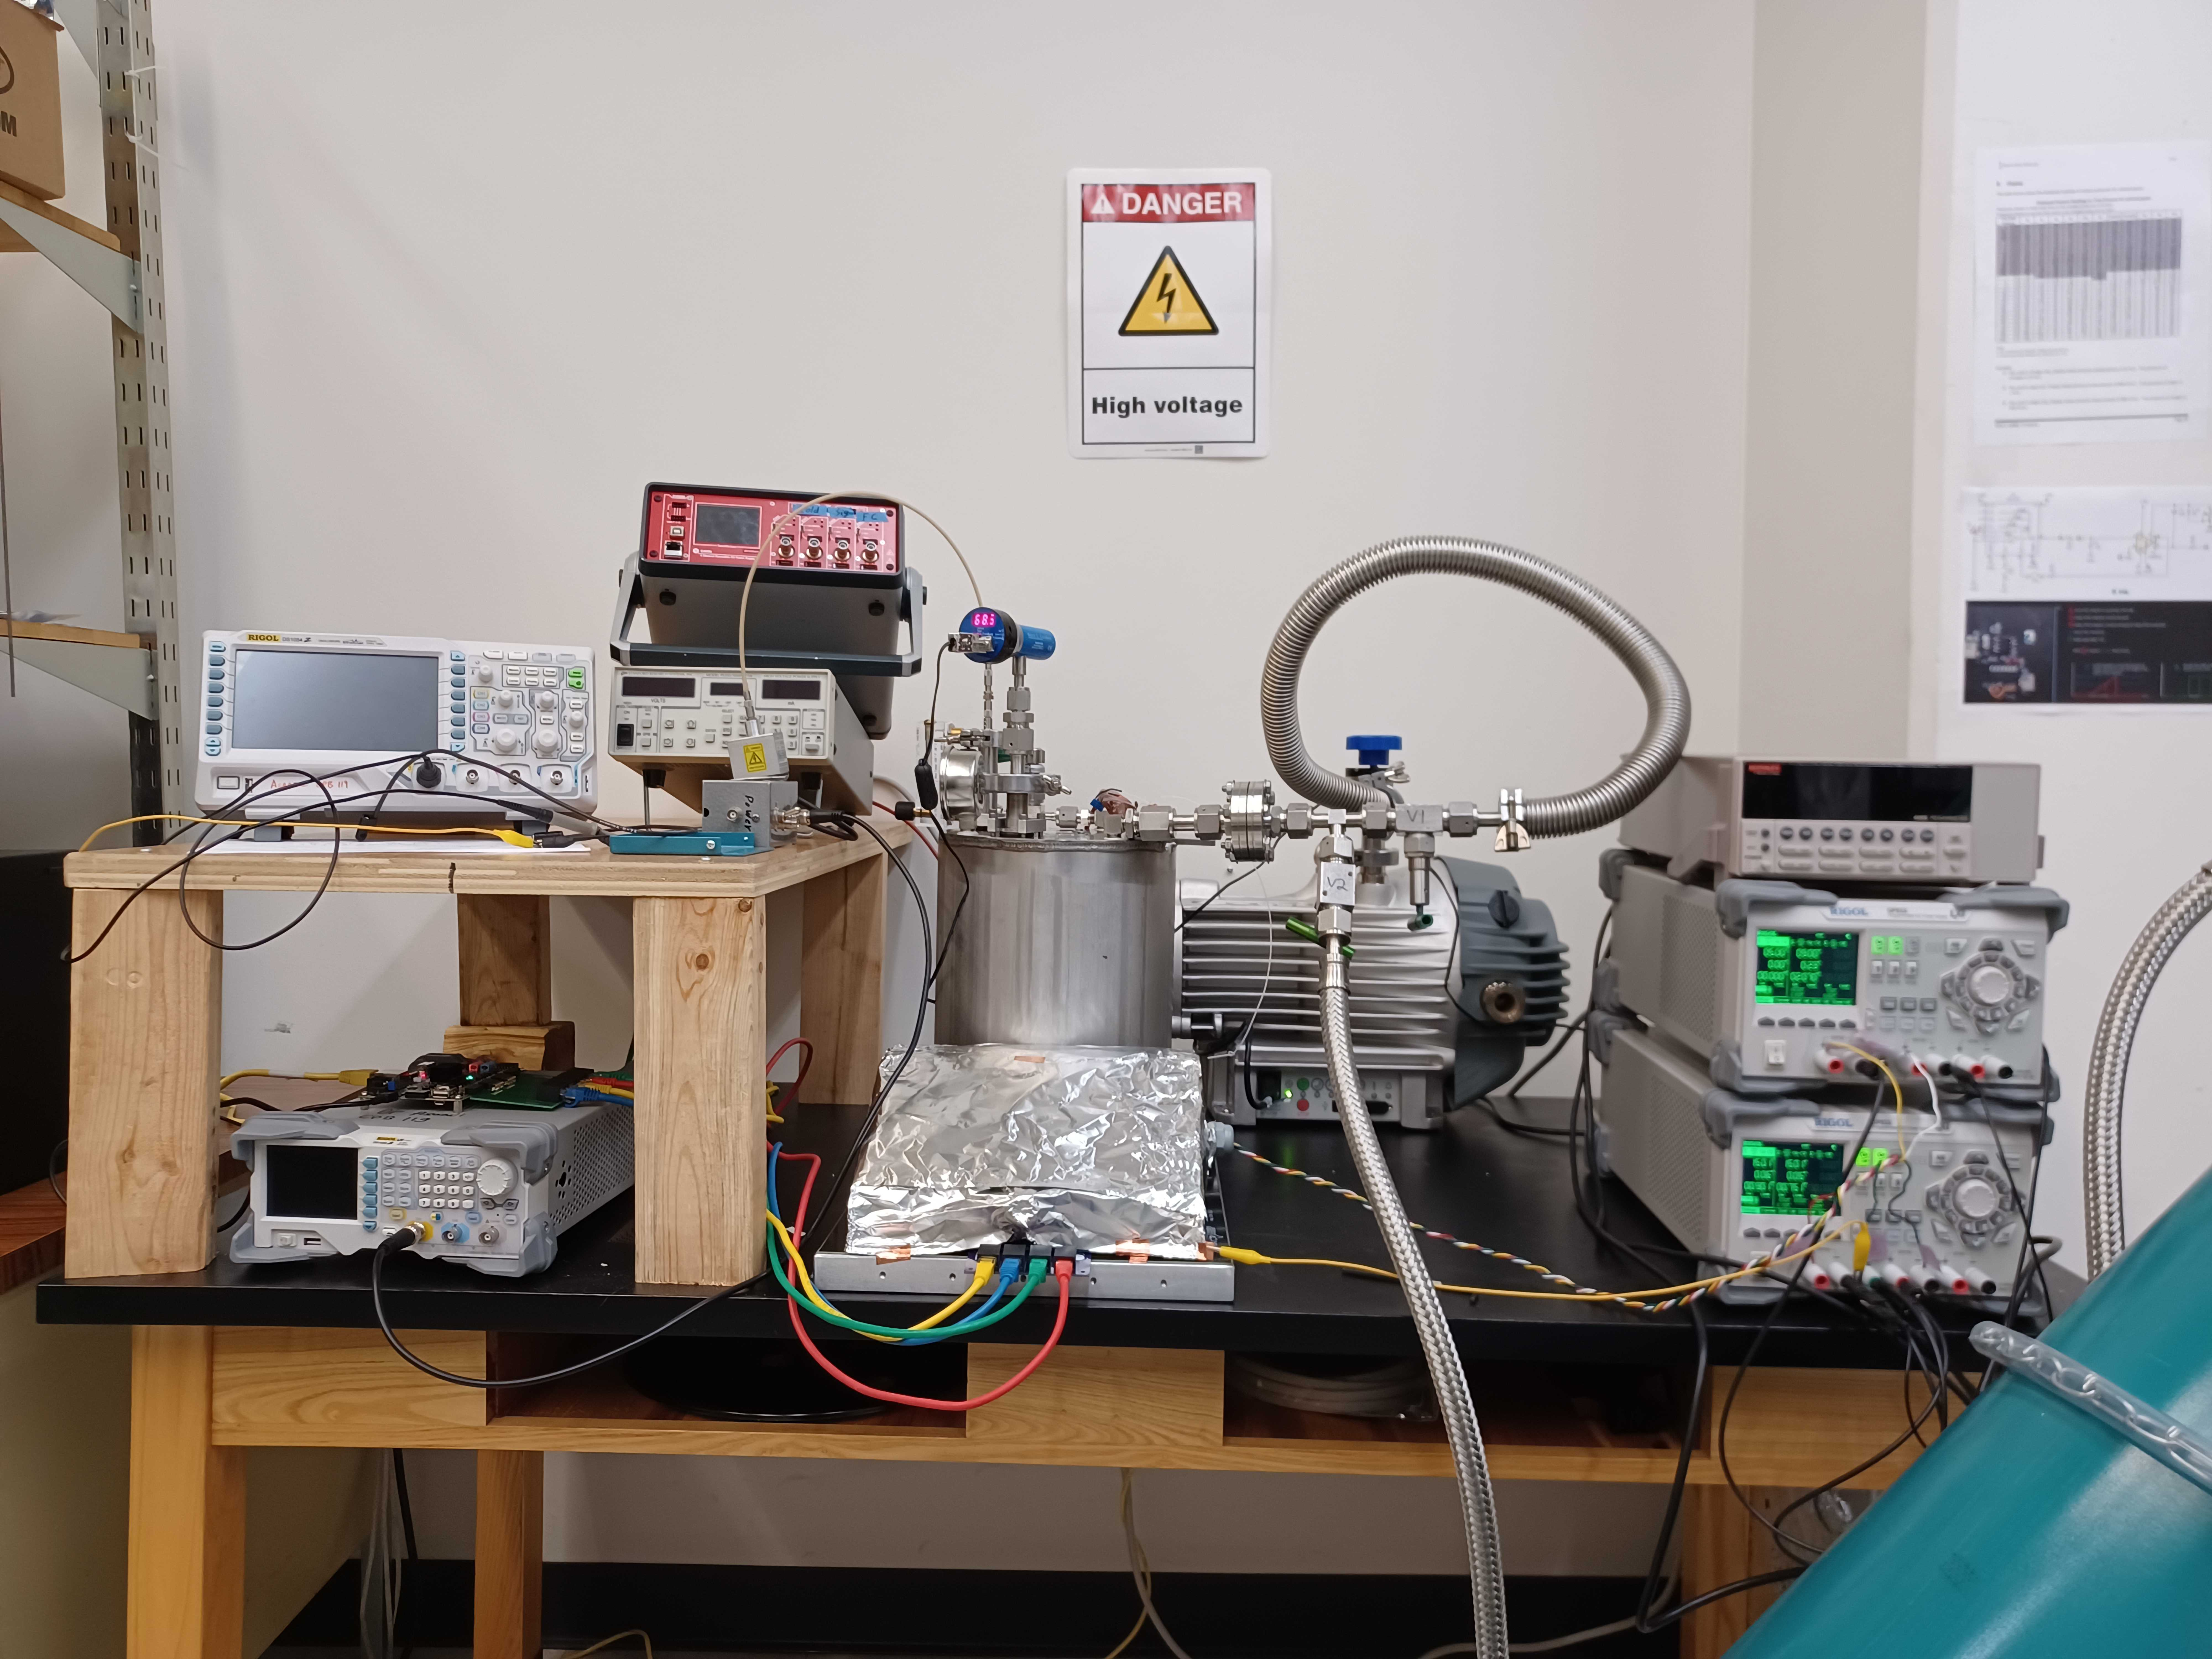
\includegraphics[width=\textwidth]{images/SAQ_physical_setup.jpg}
\caption{The SAQ setup at UTA.
In the center is the TPC, SAQ board~(Figure~\ref{fig:saq_readout_board}), and pump as shown in Figure~\ref{fig:saq_physical_setup_flatten}.
}
\label{fig:saq_setup_flatten}
\end{figure}

\begin{figure}[]
\centering
\begin{subfigure}{.5\textwidth}
  \centering
  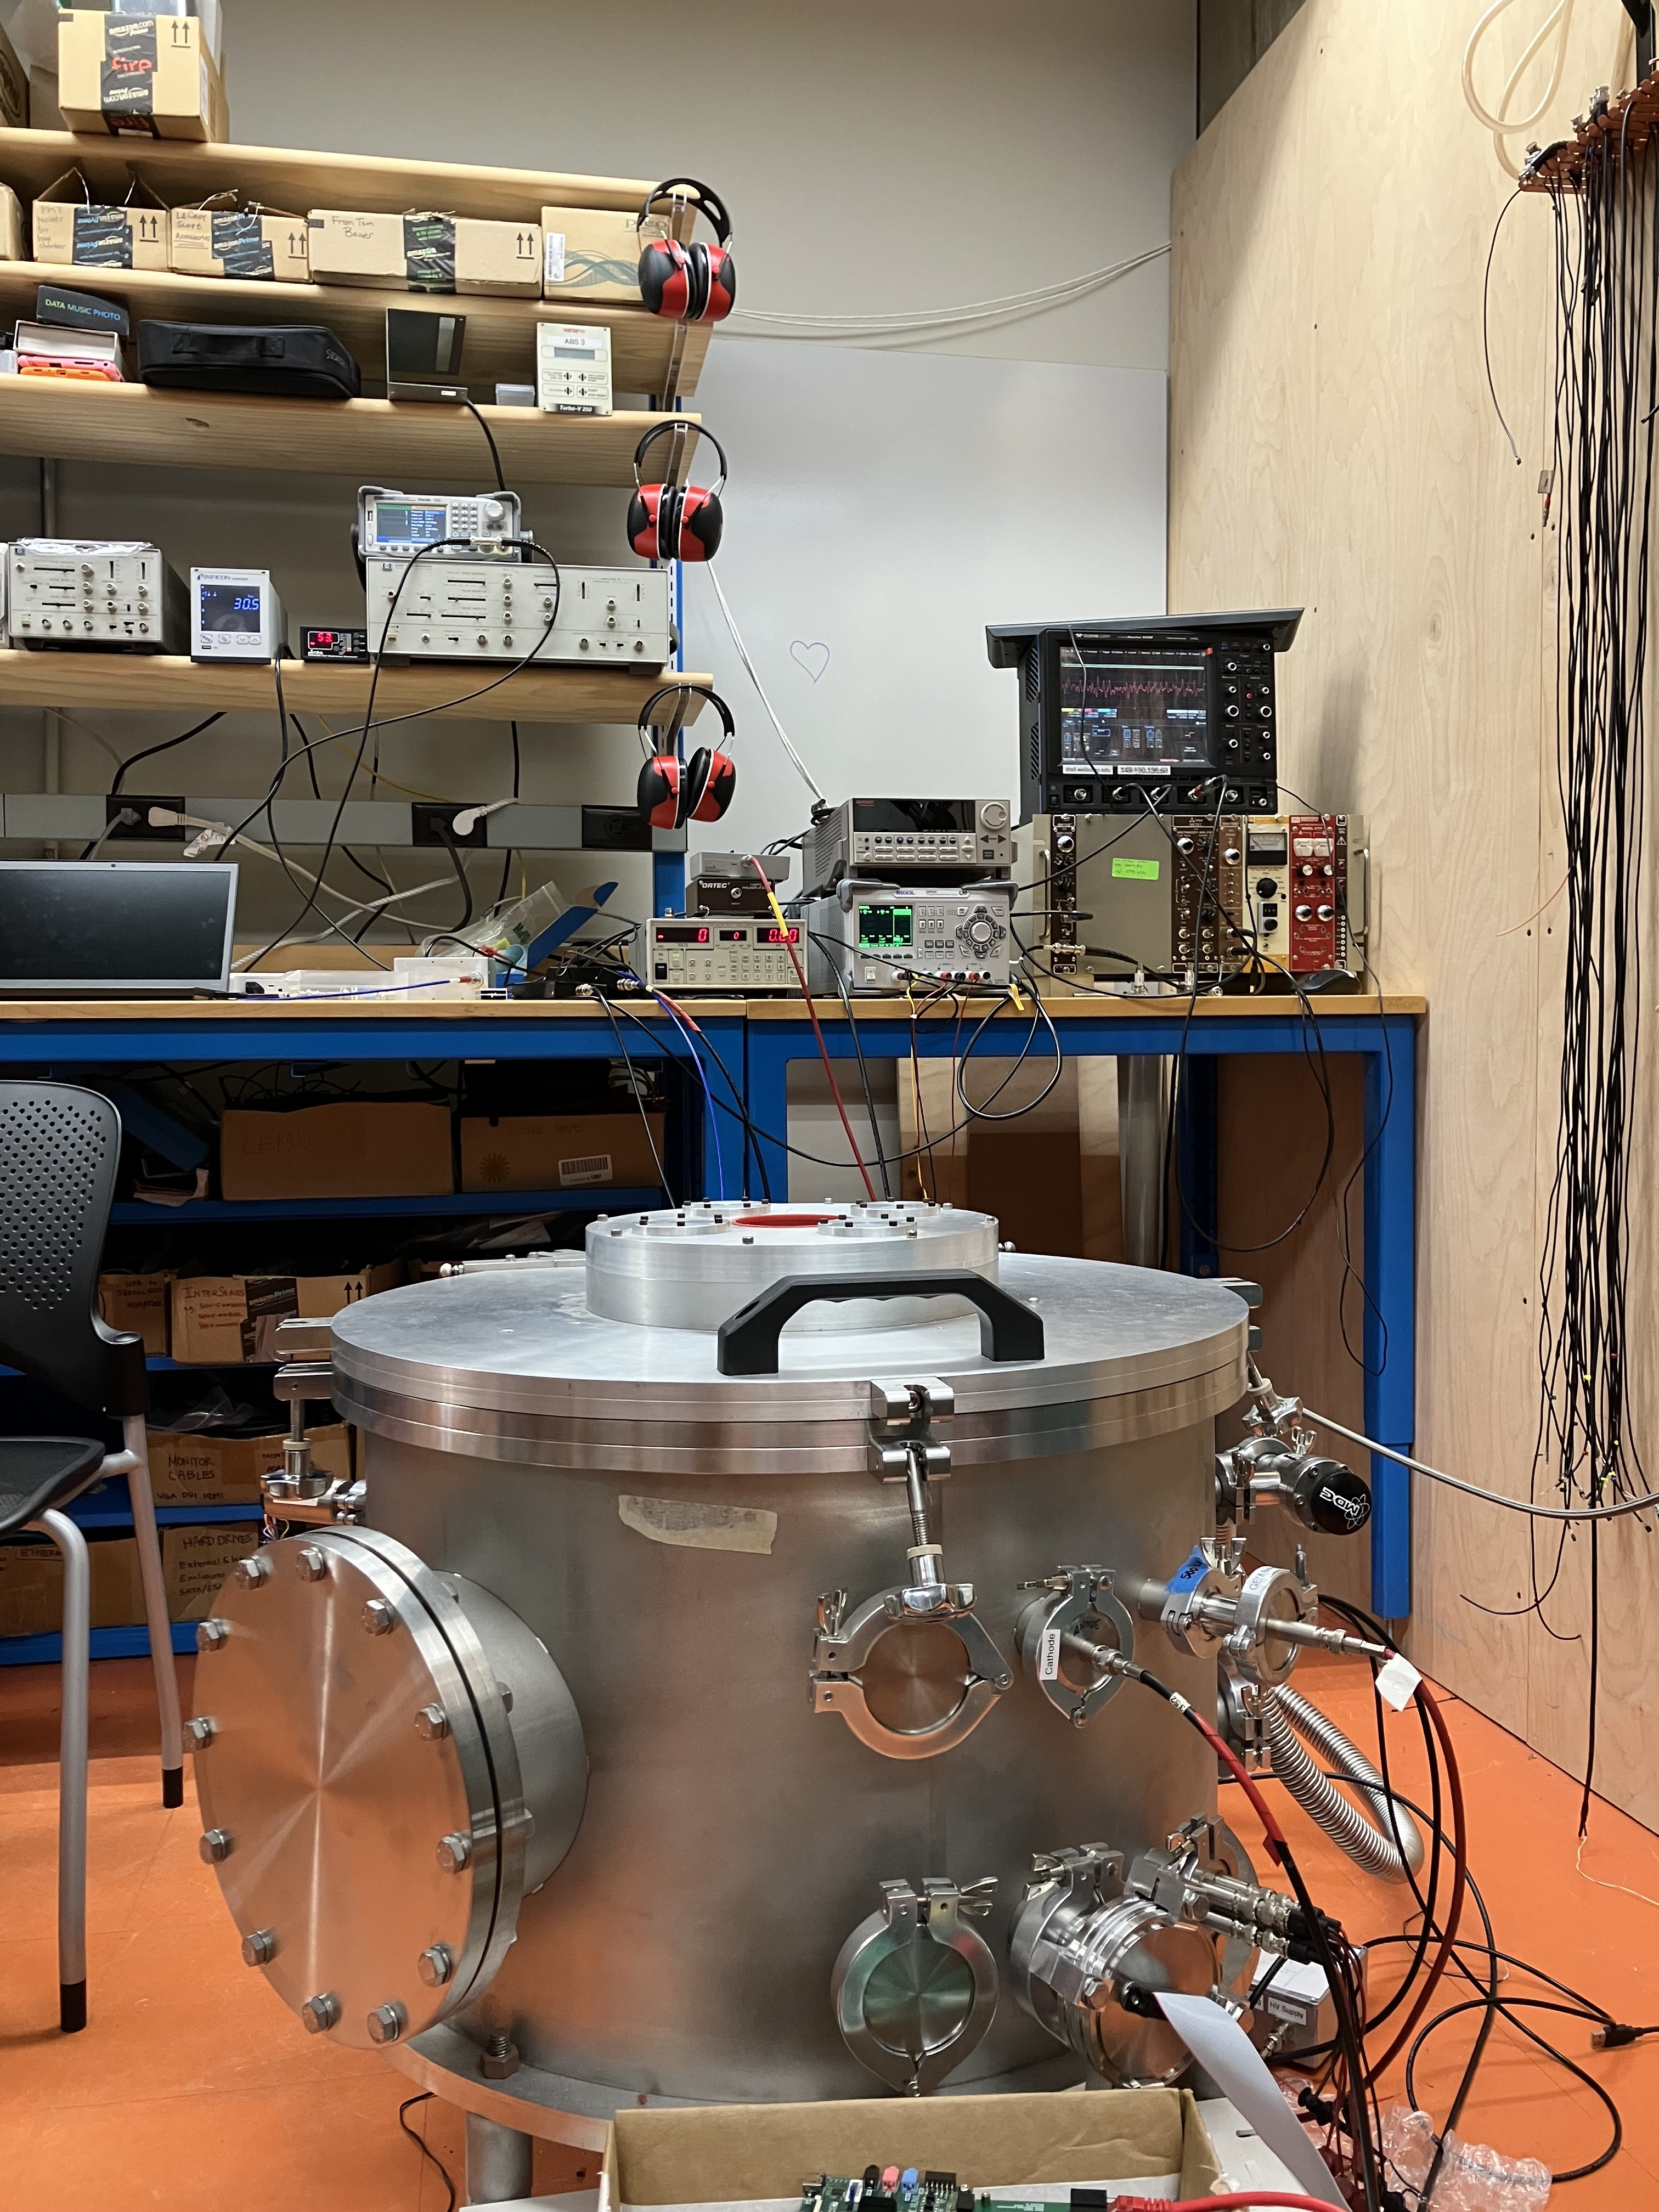
\includegraphics[width=\textwidth]{images/saq_wellesley_tpc.jpg}
  \caption{}
\end{subfigure}%
\begin{subfigure}{.5\textwidth}
  \centering
  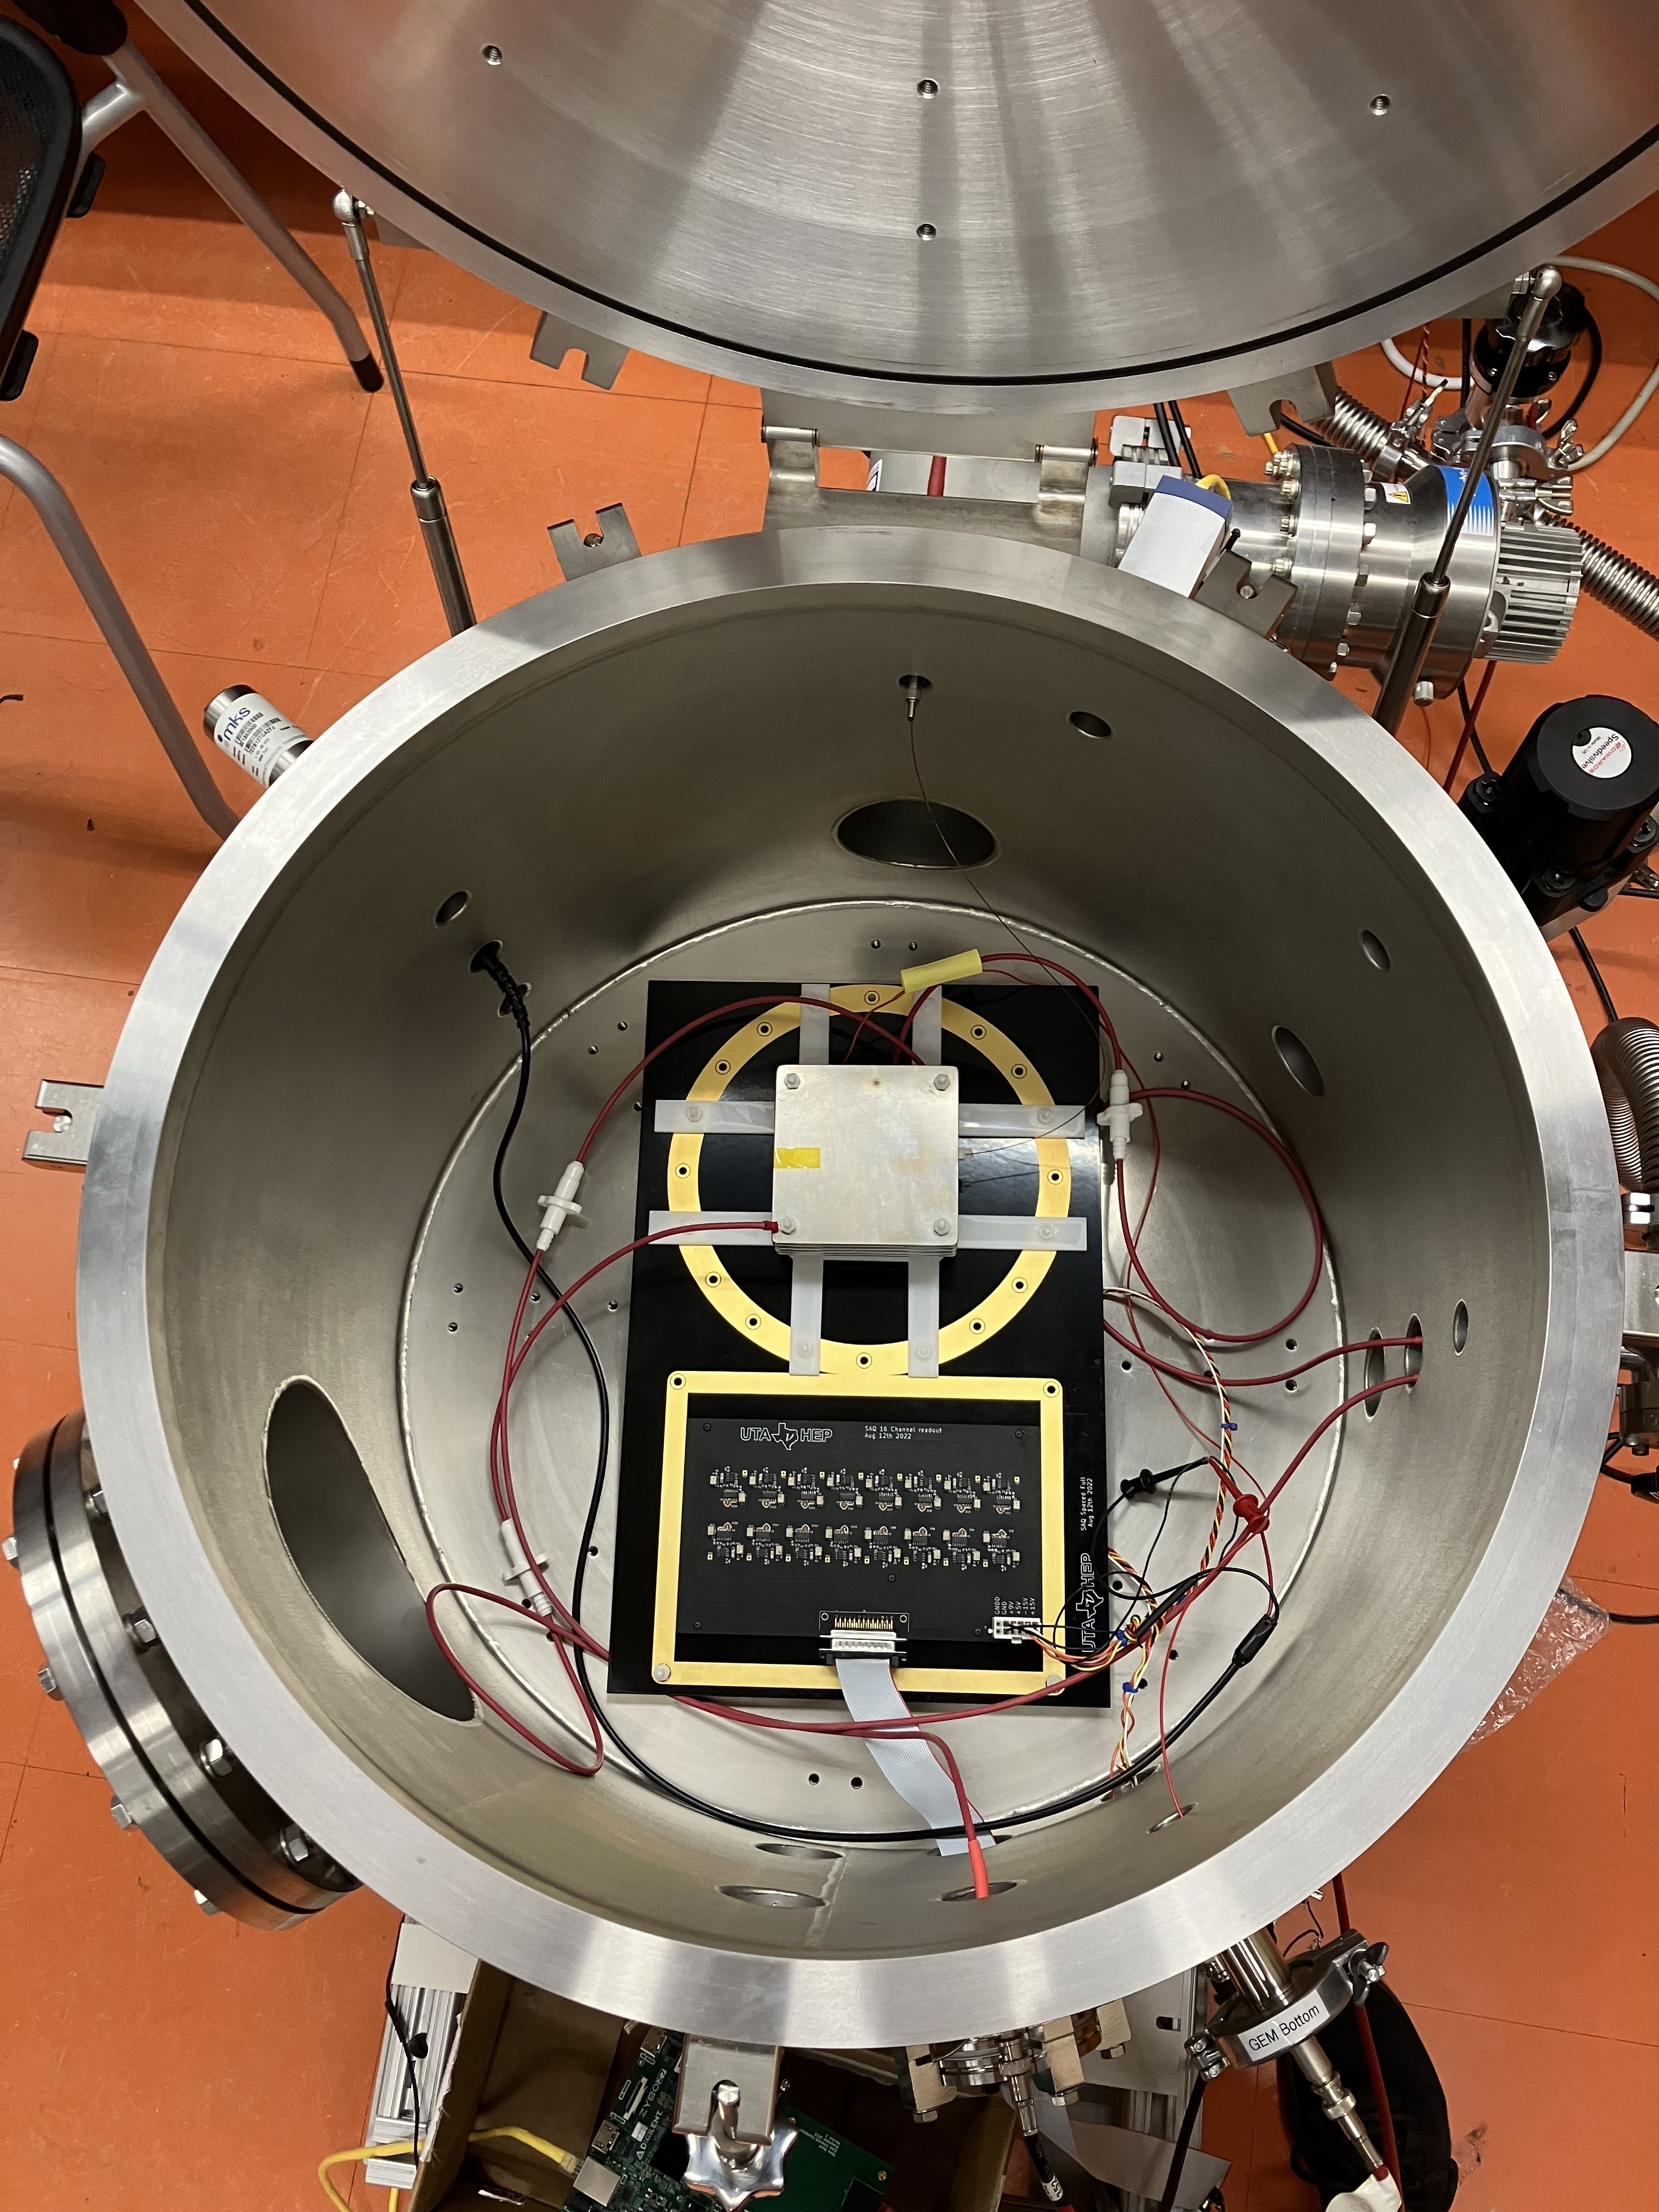
\includegraphics[width=\textwidth]{images/saq_wellesley_tpc_daq.jpg}
  \caption{}
\end{subfigure}
\caption{Picture of the TPC and DAQ setups at Wellesley University.
Image of the TPC cage (left) is used to store P-10 Argon gas. P-10 Argon gas uses a 10\% mixture of methane, and prevents sparking from the high-voltage of the TPC.
Inside of the TPC (right) shows the SAQ readout board.
The SAQ readout board is used at both UTA and Wellesley.
}
\label{fig:wellesley_tpc}
\end{figure}

The source of the electrons is a gold foil and a Hamamatsu L13651~\citep{hamamatsu_tls1023e} Xenon Gas Lamp which removes the electrons via the photo-electric effect~\citep{https://doi.org/10.1002/andp.19053220607}.
As the electrons are removed from the gold, they enter the electric field and are drifted down to a collection plane.
A simplified image of the working TPC, rings, and GEM placement are shown in Figure~\ref{fig:saq_physical_setup_flatten}.
The design of the GEM PCB as well as its operating voltages is based on work presented in~\citep{THORPE2023167438}.

\begin{figure}[]
\centering
\begin{subfigure}{.45\textwidth}
  \centering
  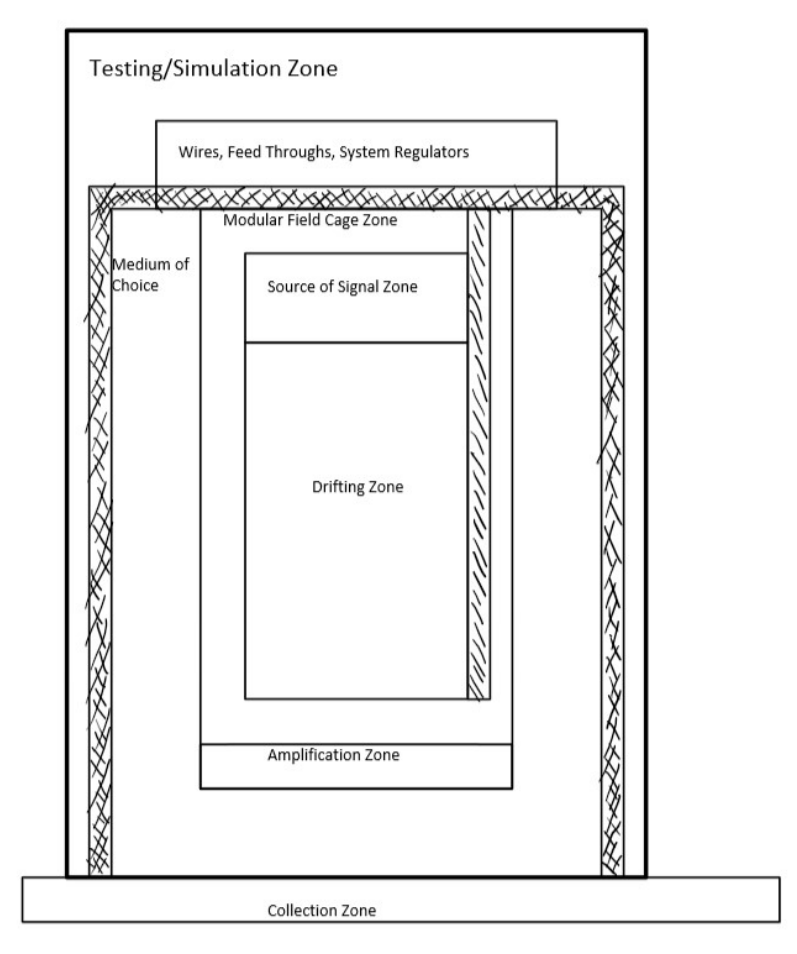
\includegraphics[width=\textwidth]{images/saq_tpc_insides.png}
  \caption{}
\end{subfigure}%
\begin{subfigure}{.38\textwidth}
  \centering
  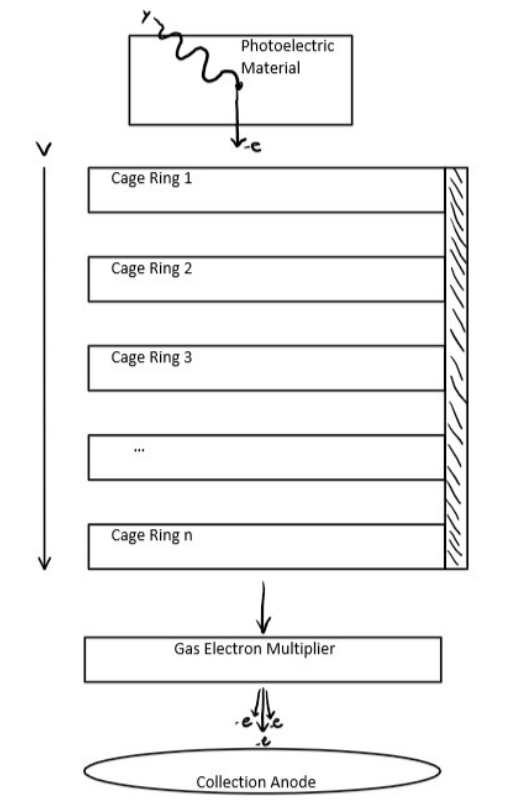
\includegraphics[width=\textwidth]{images/saq_rings_insides.png}
  \caption{}
\end{subfigure}
\caption{The SAQ model shown explicitly Figure~\ref{fig:saq_setup_flatten}.
The TPC (left) shows that the gold foil target for the flash lamp target is at the top of the detector.
Electrons are removed and drifted through the rings (right) of the TPC.
The rings are separated by $\approx 0.84~\unit{cm}$, where they encounter an average drift field of 500~\unit{\frac{V}{cm}}.
}
\label{fig:saq_physical_setup_flatten}
\end{figure}


\subsection{The Integrator Circuit}

The integrator circuit used in the SAQ experiment is shown in Figure~\ref{fig:saq_circuit_kicad}.
The Integrated Circuit (IC) used is the IVC-102~\citep{ivc_datasheet}, where the selected capacitor is 10~\unit{pF}.
We selected the lowest available capacitance of the IVC chip in order to ensure that resets are produced with the lowest amount of possible charge~\ref{eq:capacitor}.
Further configuration of the charge required per reset uses a configurable voltage (VDD in Figure~\ref{fig:saq_circuit_kicad}) with a variable resistor.
Charge is accumulated from the TPC as an input into the IVC chip.
The comparator sends an output pulse with a width of $\approx 10~\unit{\mu s}$ once the voltage on the IVC exceeds four times the voltage across VDD, due to the voltage divider.

\begin{figure}[]
\centering
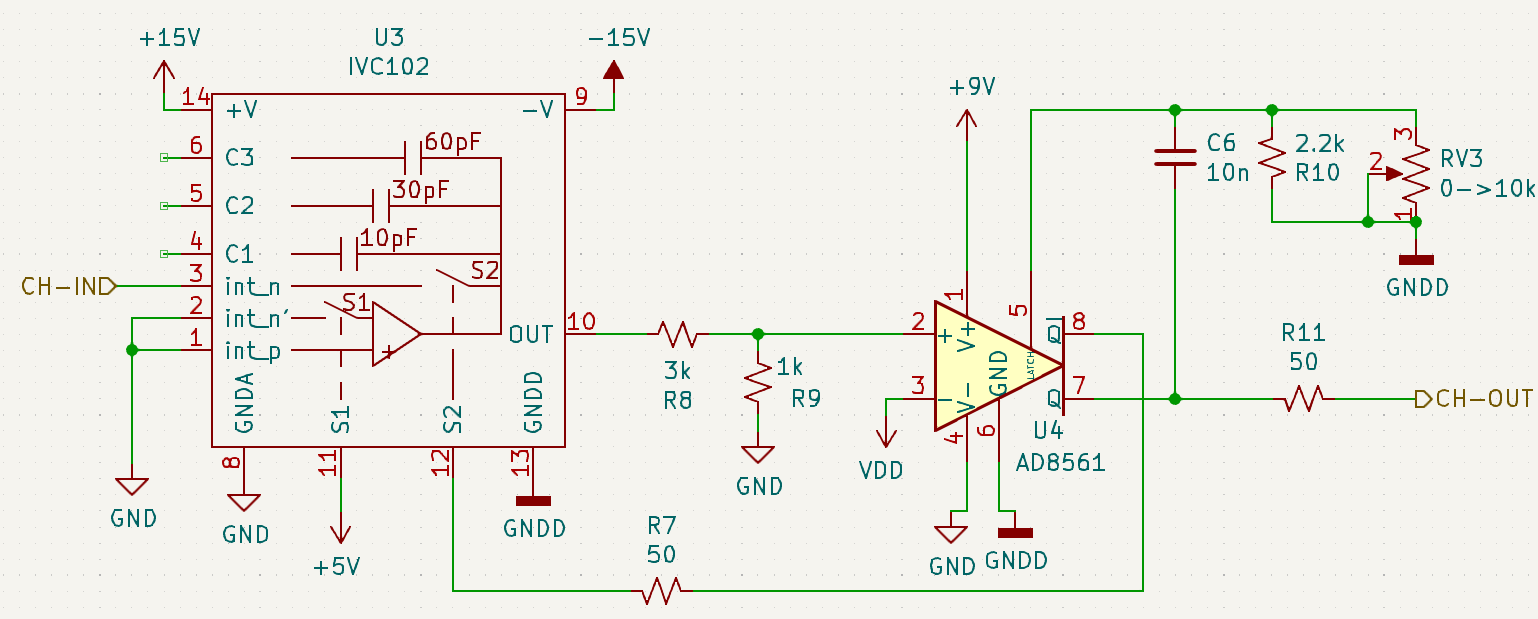
\includegraphics[width=\textwidth]{images/saq_integrator_circuit.png}
\caption{
A schematic of the front-end CSA and trigger components.
The IVC~\citep{ivc_datasheet} chip chosen as the off-the-shelf integrator for this experiment.
The main selection choice for this part is due to its low input bias current $\ll 750~\unit{fA}$.
}
\label{fig:saq_circuit_kicad}
\end{figure}

\begin{figure}[]
\centering
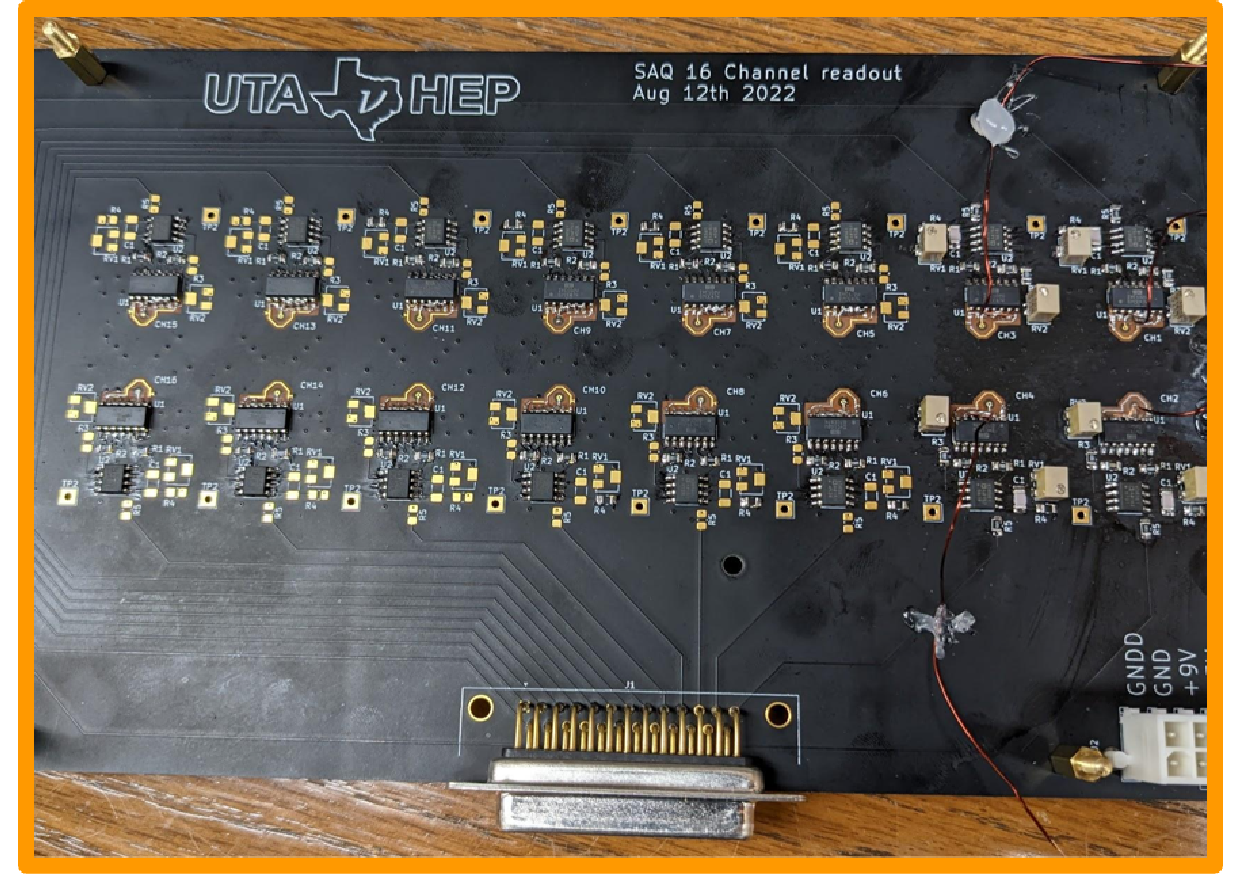
\includegraphics[width=\textwidth]{images/SAQ_16_ivc_readout_board.pdf}
\caption{The SAQ front-end board of 16 input IVC channels.
Each of the 16 channels are based on Figure~\ref{fig:saq_circuit_kicad}.
}
\label{fig:saq_readout_board}
\end{figure}

Two different collection plane geoemtries are tested.
The two different geometries change the amount of exposed copper and are shown in Figure~\ref{fig:trace_boards}.
The "thin" trace (right image) board exposes 6~\unit{mm} wide copper rings around the center of the TPC
The "thick" trace board inverts the silt-screen and exposed copper and instead separates the collection rings by 6~\unit{mm} wide silt-screen traces.

\begin{figure}[]
\centering
\begin{subfigure}{.45\textwidth}
  \centering
  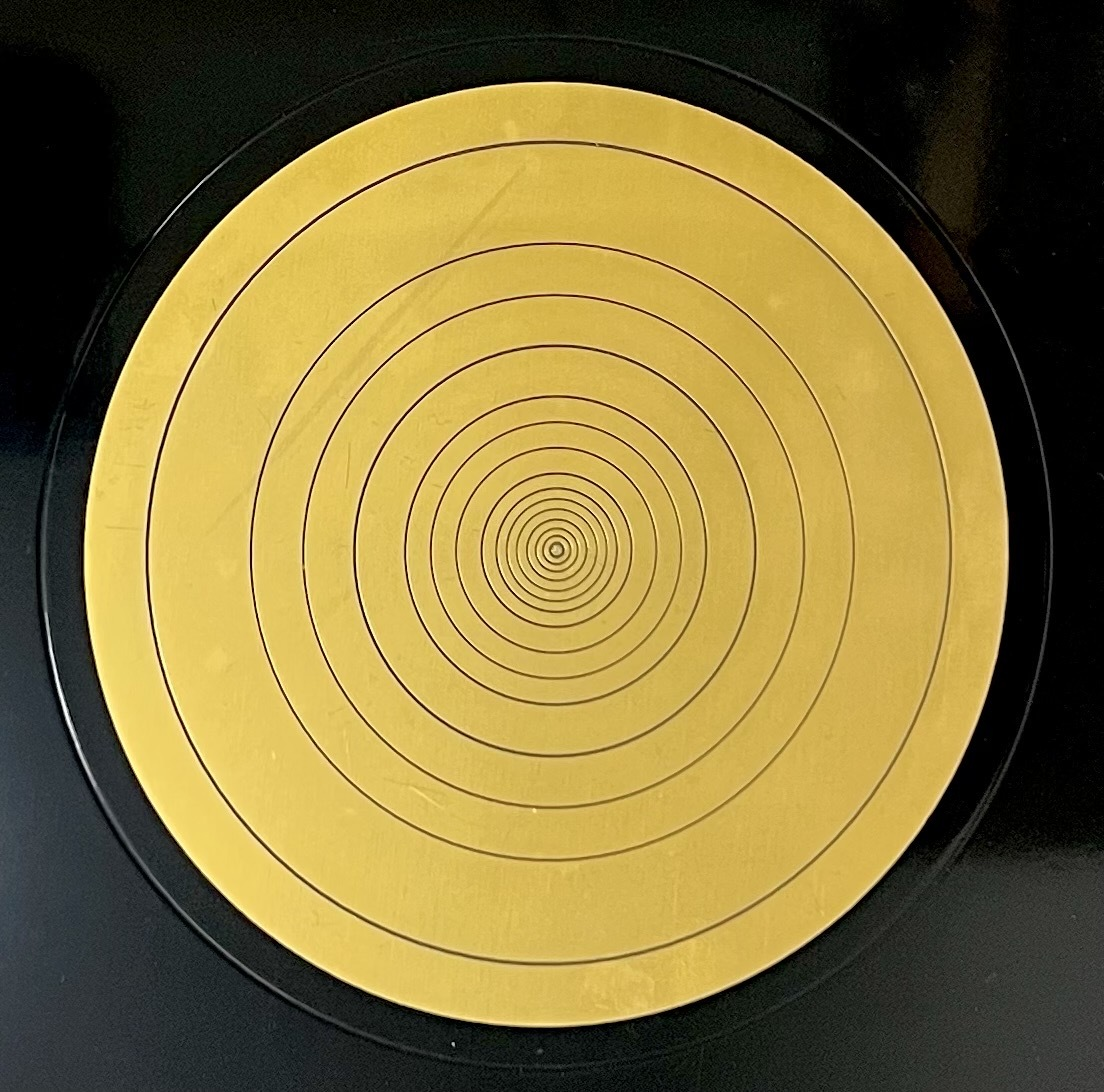
\includegraphics[width=\textwidth]{images/thick_board_example.jpg}
  \caption{}
\end{subfigure}%
\begin{subfigure}{.45\textwidth}
  \centering
  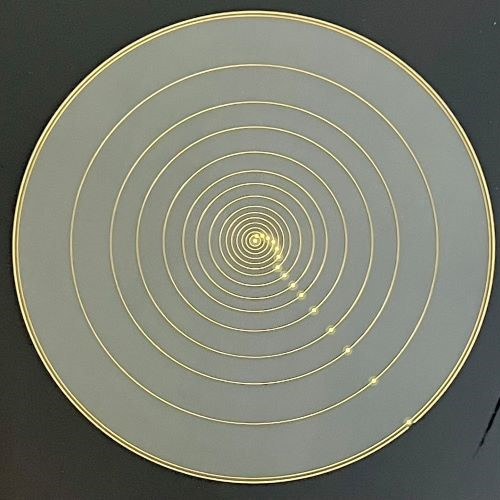
\includegraphics[width=\textwidth]{images/thin_trace_board_example.jpg}
  \caption{}
\end{subfigure}
\caption{Different Trace Boards used in the SAQ Experiment.
The thick trace board (left) differs from the thin trace board (right) in that most of the surface area in the field cage can collect electrons.
The thin (right) trace board replaces the collection rings with silt-screen, and the silt-screen with collection rings.
Because the traces are so small, vias are used to connect the thing collection rings to the input of the integrator.
}
\label{fig:trace_boards}
\end{figure}

An example of resets produced from the integrator circuit is shown in Figure~\ref{fig:saq_resets}.
Each reset corresponds to a charge accumulation of $\approx 10~\unit{pC}$.
The time difference between each reset shown is equivalent to the amount current accumulated at the IVC~(Equation~\ref{eq:irecon}).
A simplified diagram of how the reset time differences are recorded is shown in Figure~\ref{fig:saq_reconstruction}.

\begin{figure}[]
\centering
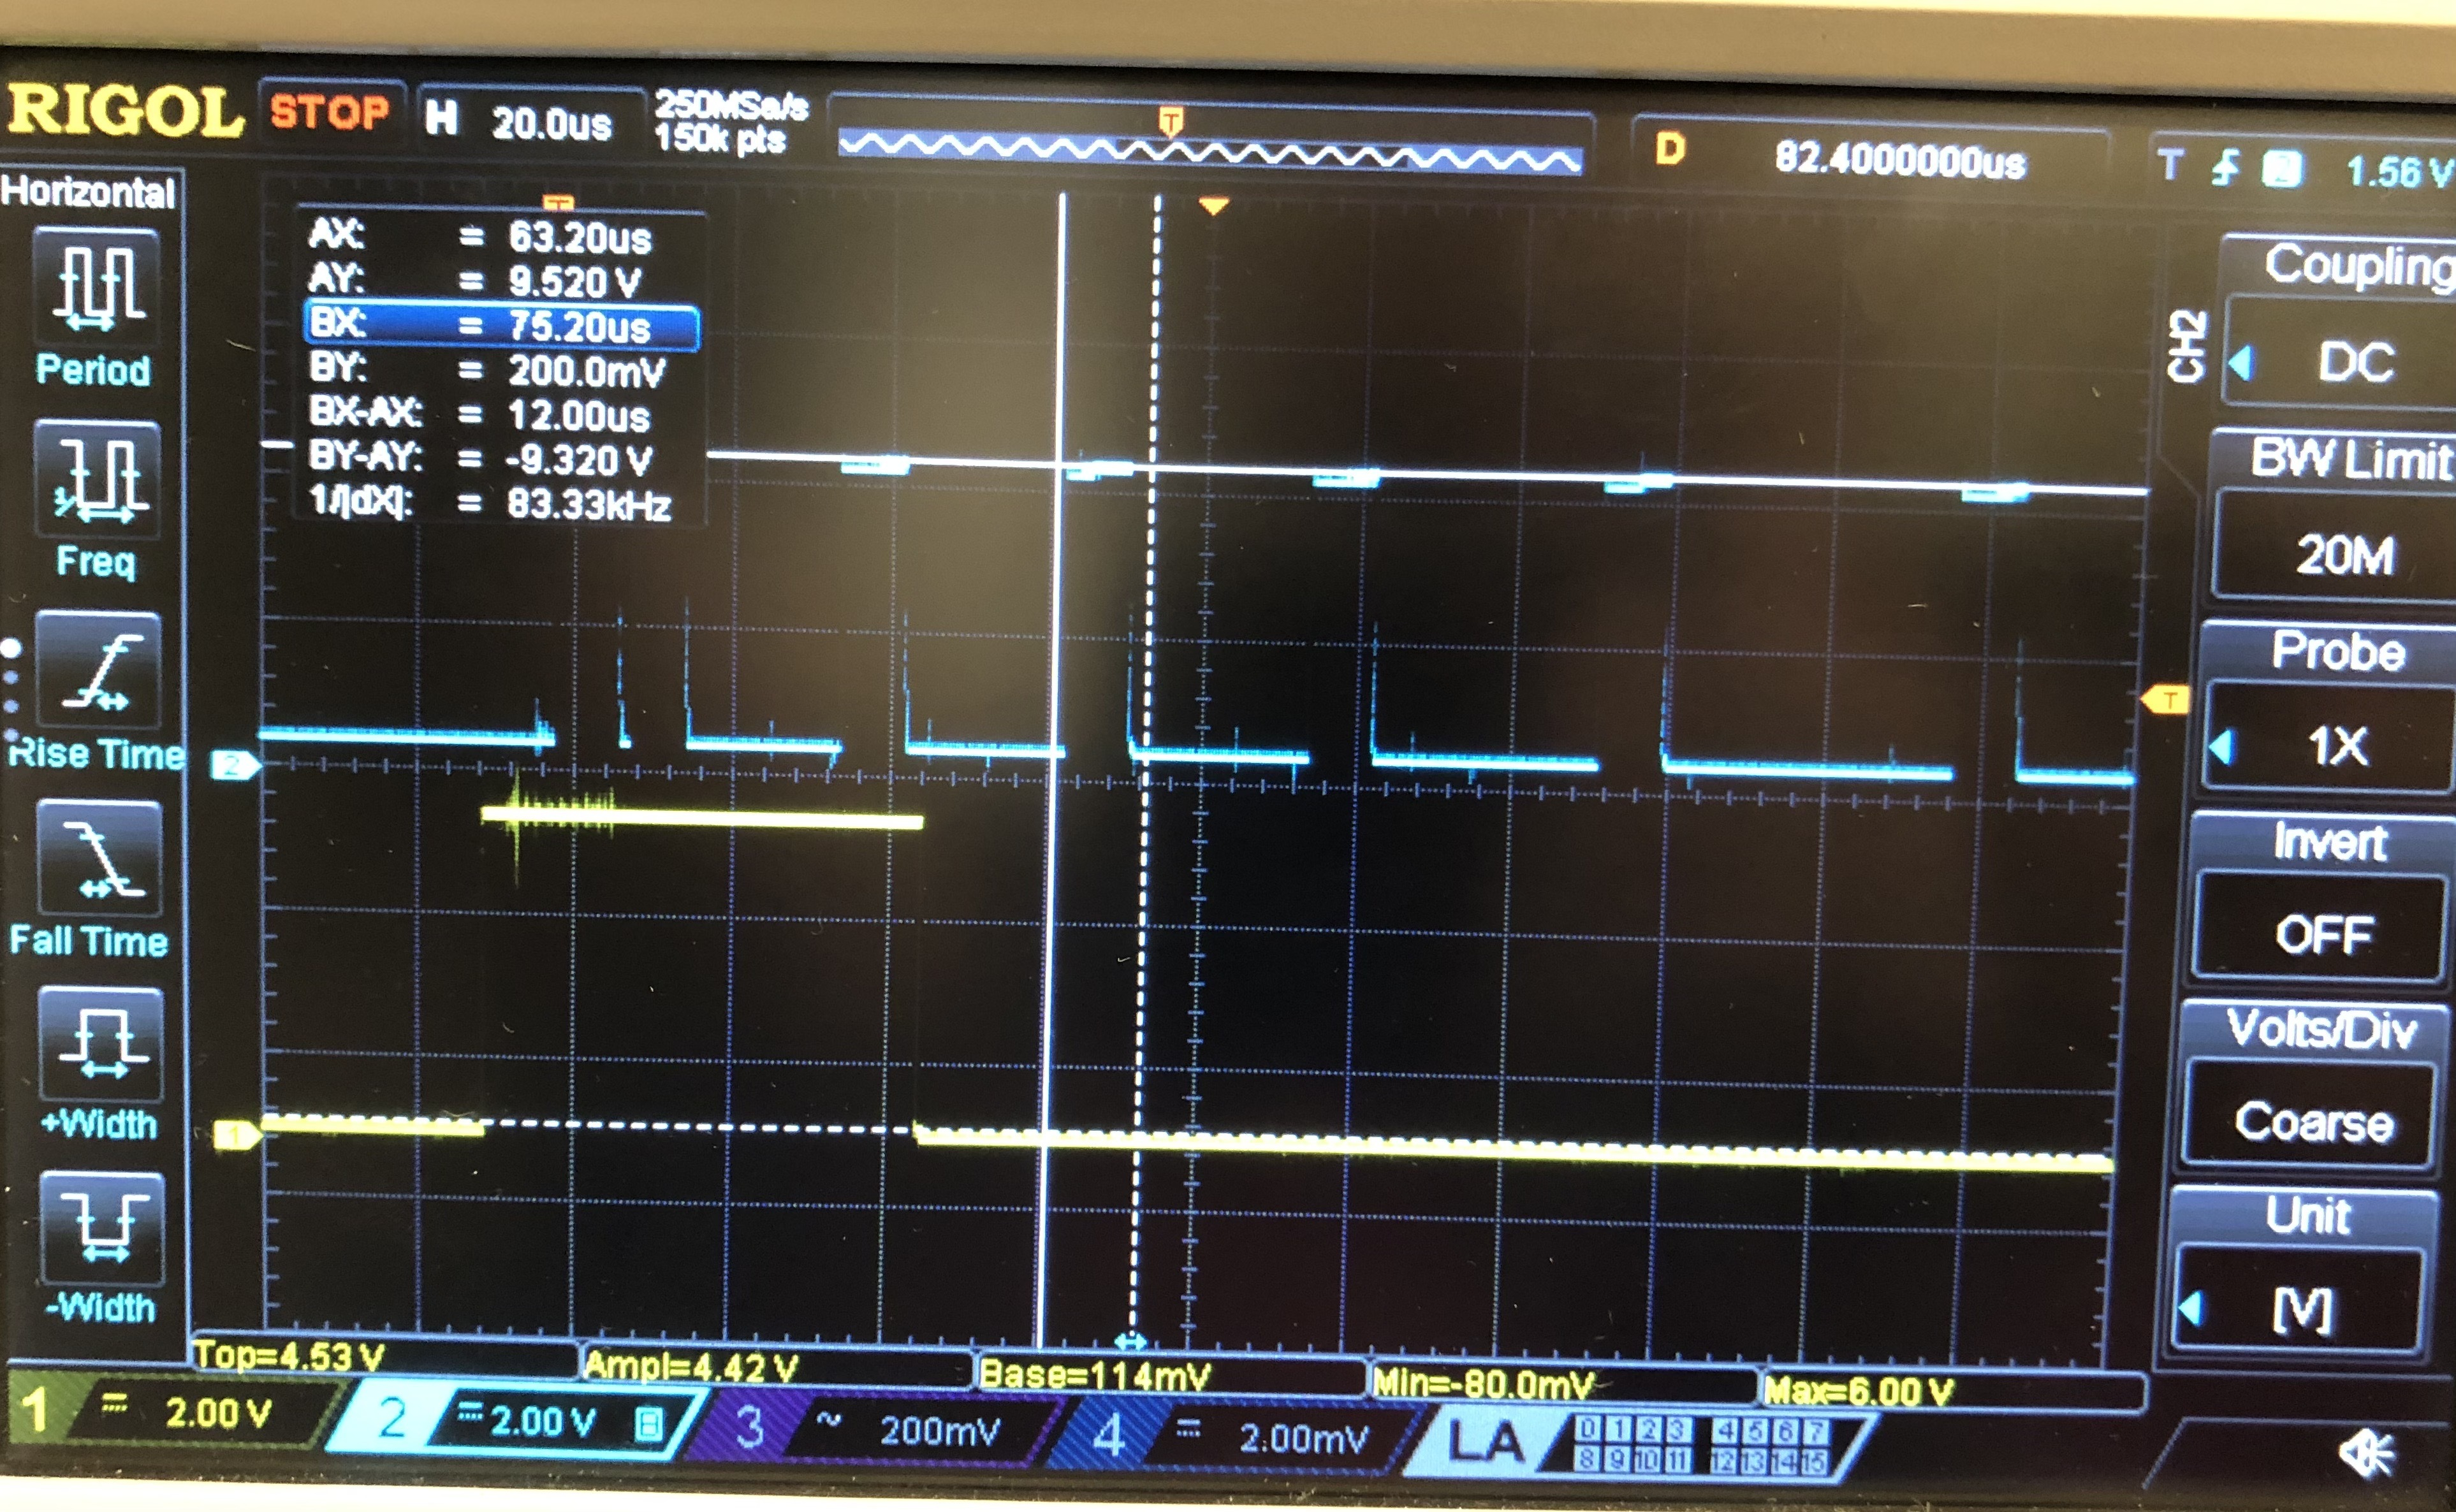
\includegraphics[width=\textwidth]{images/saq_reset_pulse_gem_thickBoard.jpg}
\caption{Waveform measurements of the trigger sent to the Xenon Flash lamp (yellow, bottom), and the reset pulse responses sent by the comparator.
Each reset corresponds to a build up of $\approx 10~\unit{pC}$ of charge stored up on the IVC capacitor.
Seen in the waveform is a decaying amount of charge buildup on the capacitor, which is reflected in the increasing time separation between successive resets.
}
\label{fig:saq_resets}
\end{figure}

\begin{figure}[]
\centering
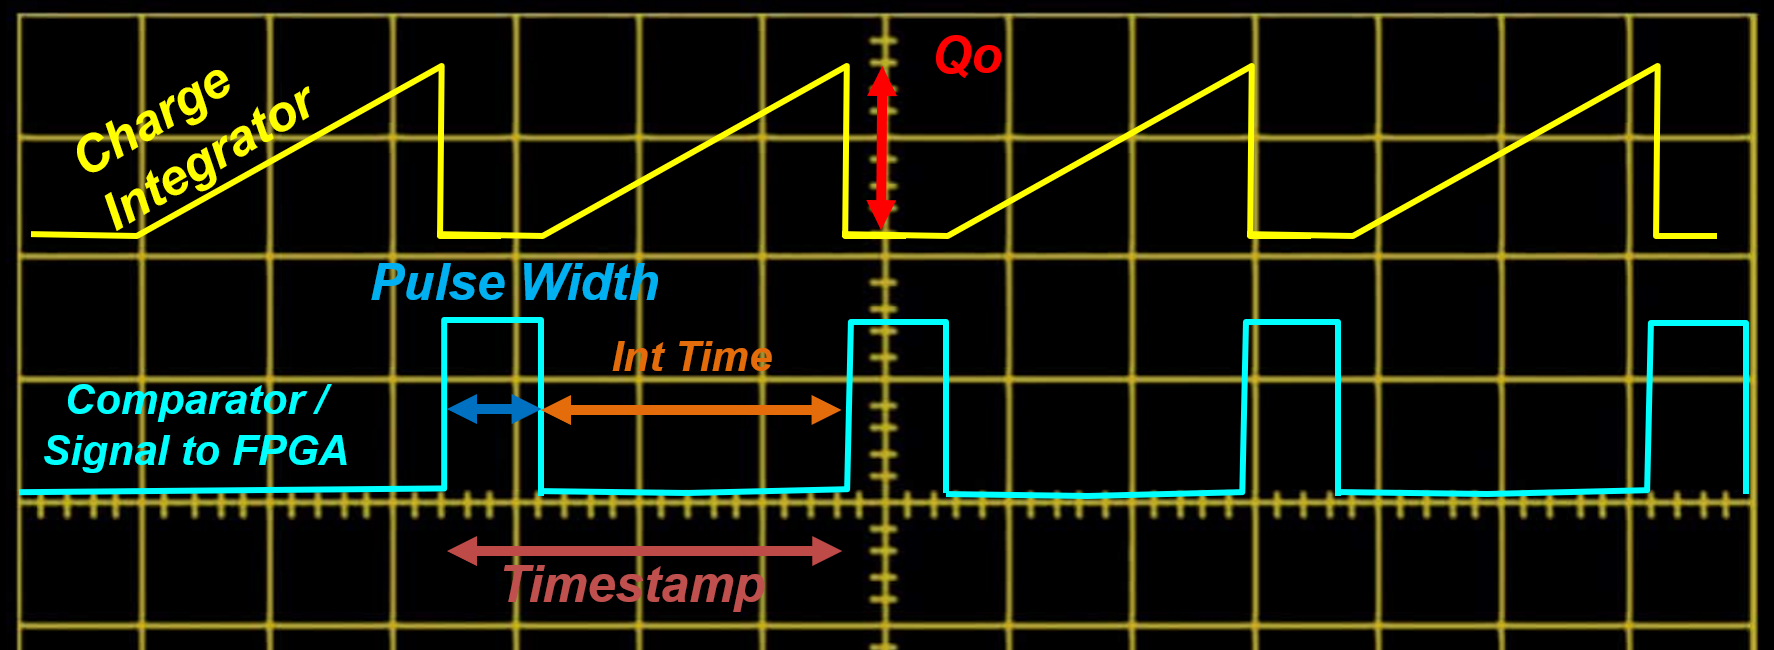
\includegraphics[width=\textwidth]{images/saq_example_reconstruction.png}
\caption{}
\label{fig:saq_reconstruction}
\end{figure}


\section{Data Acquisition}

All resets are recorded via a Zybo-Z7-20 Digilent FPGA prototype board, which uses an Artix Zynq-7000 based CPU archticture.
The reference manual for the Zybo Z7 board used in SAQ can be found at~\citep{zybo_zy_reference}.

\begin{figure}[]
\centering
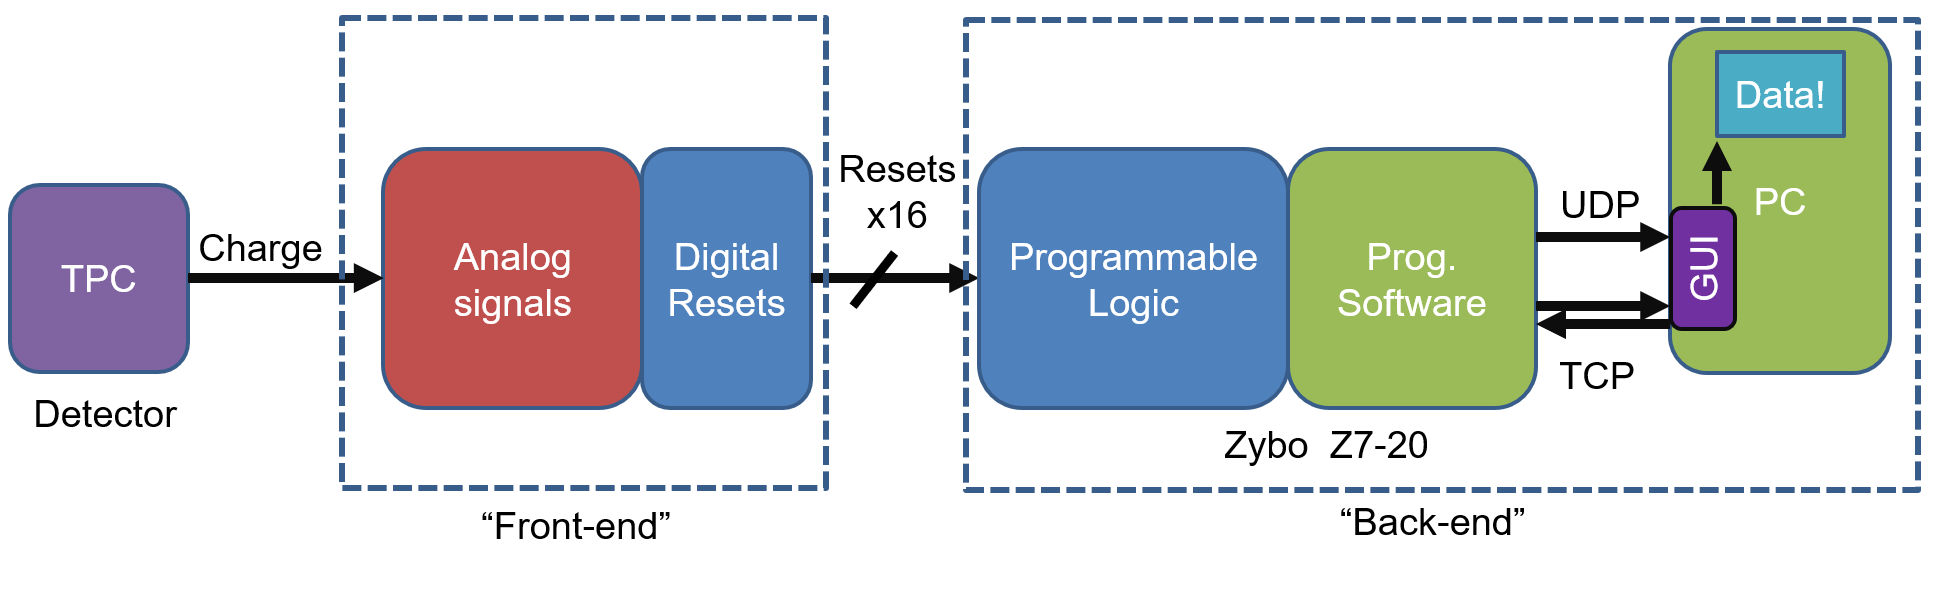
\includegraphics[width=\textwidth]{images/saq_daq_back-end_summary.png}
\caption{SAQ system over view connecting the front-end and back-end parts of a Q-Pix readout.
Gaseous Argon is used for the drift medium of the TPCs at both UTA and Wellesley.
Accumulated charge is read by the front-end which consists of 16 integrating amplifiers each connected to a comparator used as a trigger~\ref{fig:saq_circuit_kicad}.
The back-end board is a Digilent Zybo-Z7-20~(Figure~\ref{fig:saq_zybo}).
}
\label{fig:saq_diagram}
\end{figure}

\begin{figure}[]
\centering
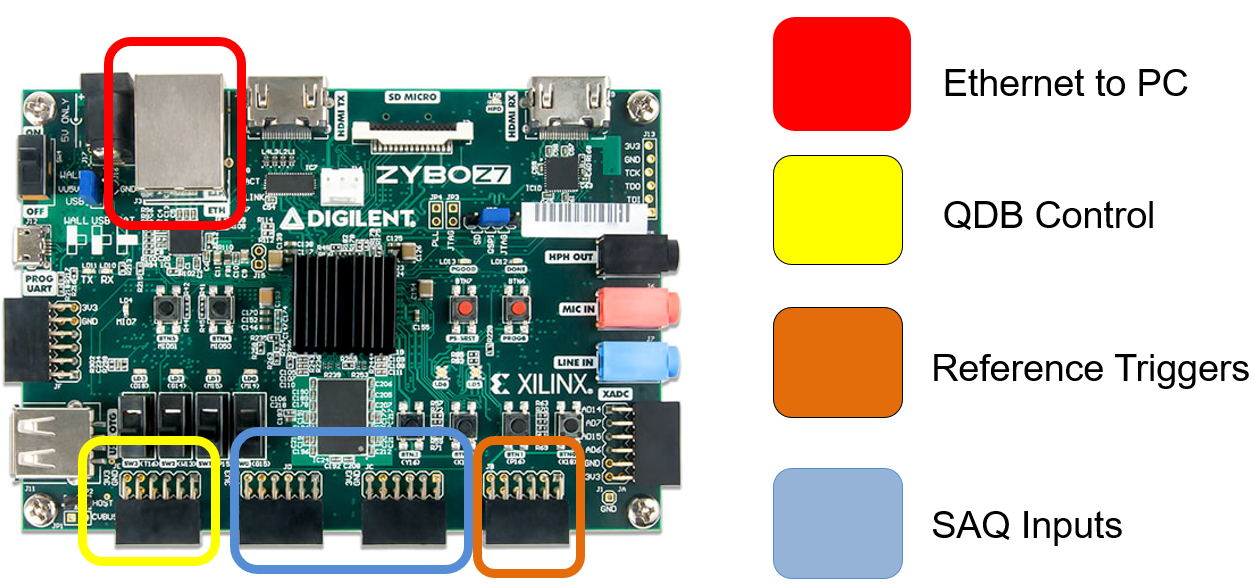
\includegraphics[width=\textwidth]{images/saq_zybo_io_summary.png}
\caption{An image of the data acquisition board from Digilent, Zybo Z7-20. 
This board was chosen for its multiple configurable input chanels, as well as the Zynq-based archiecture of the onboard FPGA.
Additionally, the use of the ethernet provides $1~\unit{GB}$ transfer speeds, which is more than sufficient for the application.
Packet data transfer rates have been verified with this readout at stable rates of 10~\unit{kHz}.
This board is also used to control the Q-Pix Digital Boards (QDB), discussed in Chapter~\ref{chap:qdb}.
}
\label{fig:saq_zybo}
\end{figure}

\begin{figure}[]
\centering
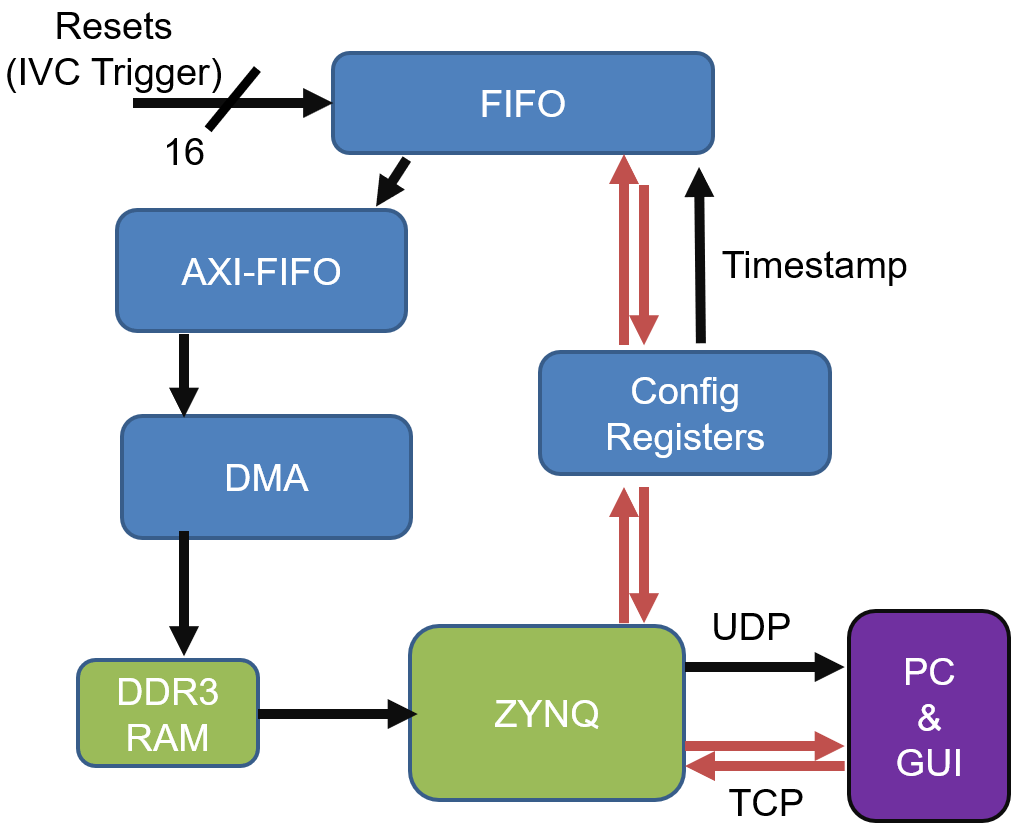
\includegraphics[width=0.5\textwidth]{images/saq_daq_firmware_summary.png}
\caption{Firmware Description}
\label{fig:saq_firmware}
\end{figure}

\begin{figure}[]
\centering
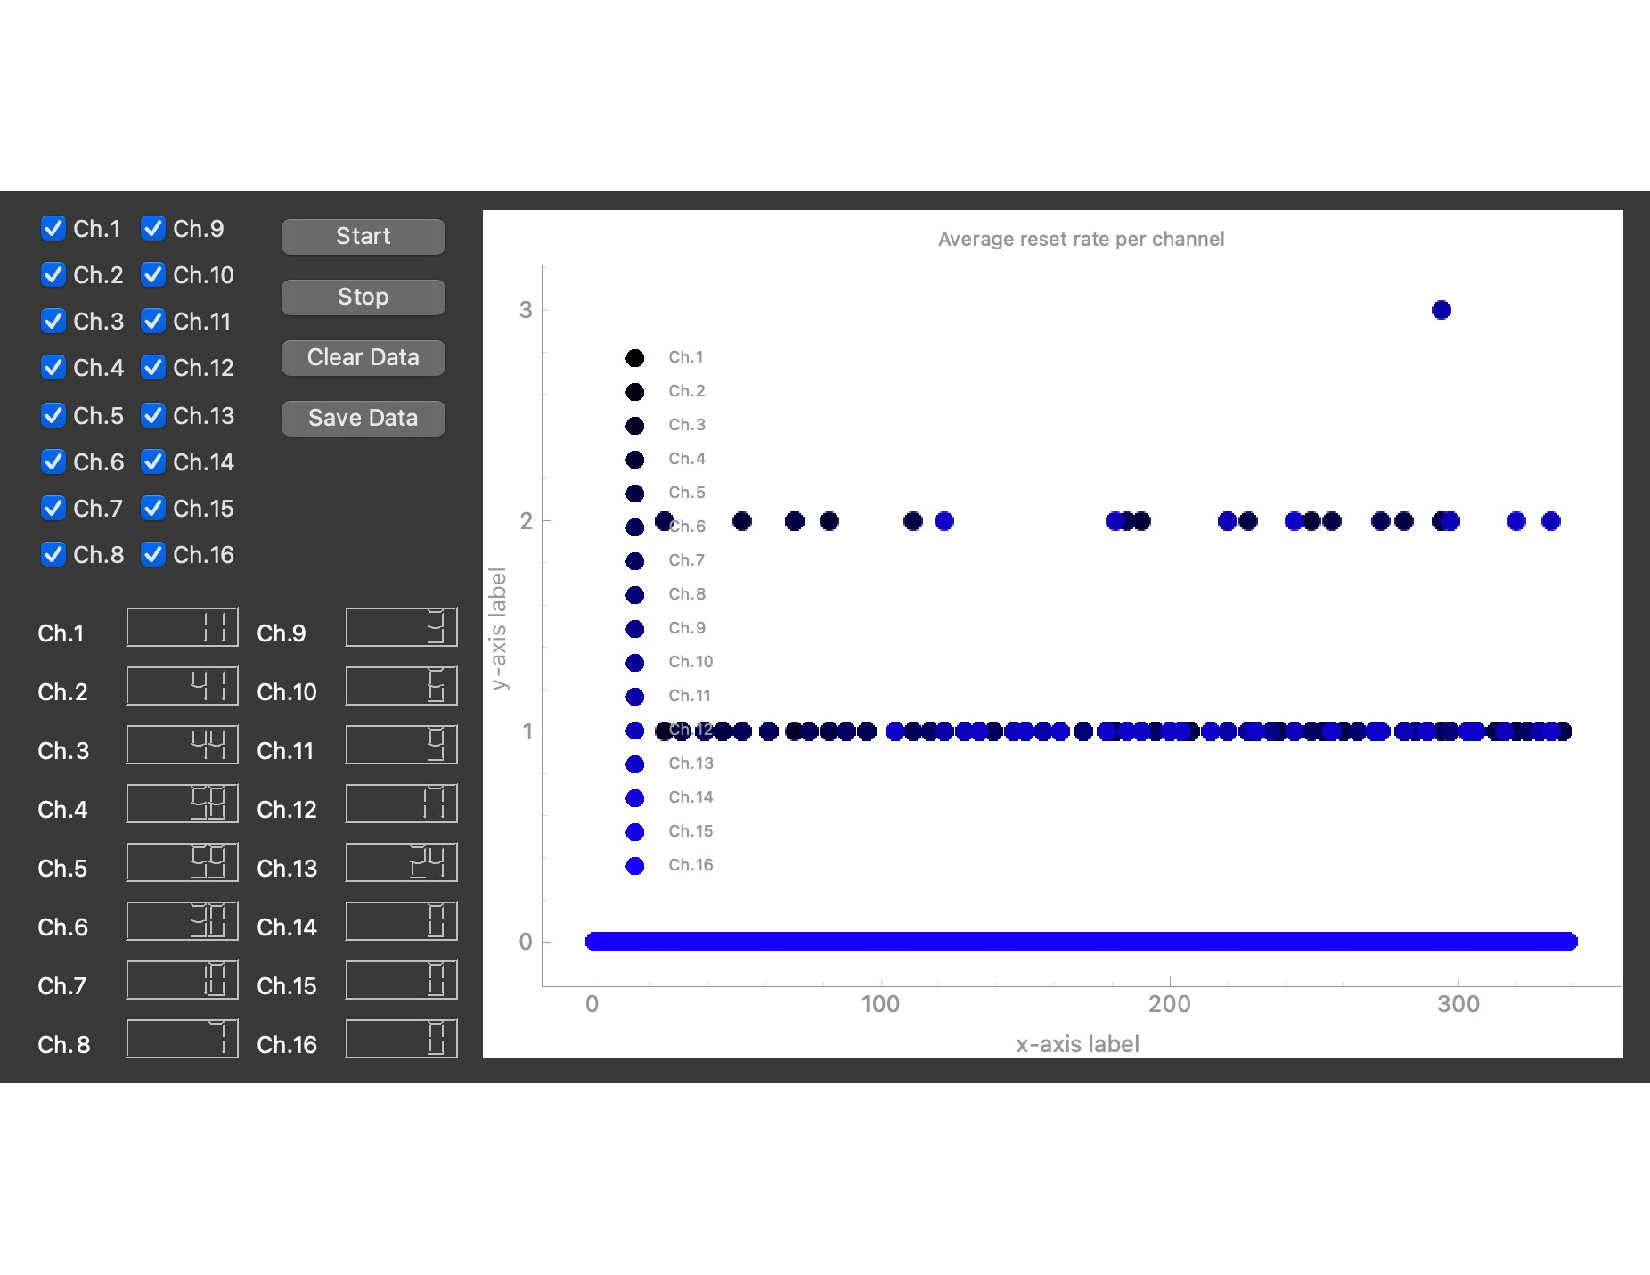
\includegraphics[width=\textwidth]{images/SAQ_gui_resets.pdf}
\caption{The SAQ GUI with real time plotting of incoming resets to the Zybo board.}
\label{fig:saq_gui}
\end{figure}


\section{Calibration Procedures}

The Q-Pix readout is dependent on two factors~(Equation~~\ref{eq:irecon_freq}): the charge and frequency calibrations.
The frequency calibration depends on the stability of the local oscillator and it's reliability to accurately record the time a timestamp occurs.
A drifting local oscillator on the digital board, the Zybo for SAQ, will cause poor reconstructions of current.
The test for the stability of the Zybo involves sending a fixed trigger (10~\unit{kHz}) into the zybo.
The reconstructed timestamp difference gives the period of the input trigger.
Figure~\ref{eq:frequency_reconstruction} shows an example of the Zybo measurements in response to a 10~\unit{kHZ} function generator with 1~\unit{ppm}.

\begin{figure}[]
\centering
\begin{subfigure}{.5\textwidth}
  \centering
  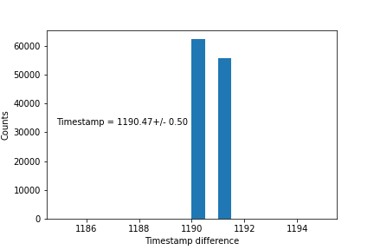
\includegraphics[width=\textwidth]{images/zybo_10khz_timestamp_frequency_calibration.png}
  \caption{}
\end{subfigure}%
\begin{subfigure}{.5\textwidth}
  \centering
  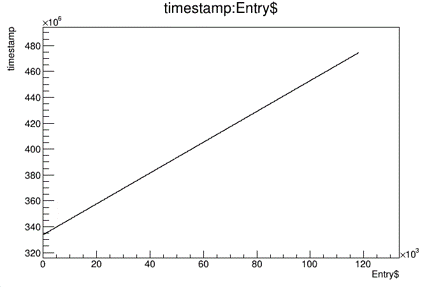
\includegraphics[width=\textwidth]{images/zybo_10khz_timestamp_graph.png}
  \caption{}
\end{subfigure}
\caption{Image of caluclated RTDs (left) between successive triggers to the zybo and the running plot of the timestamp value measured (right).
The clock period on the Zybo was reconstructed to within a single clock cycle, as shown on the left image.
The period of a 10~\unit{kHz} signal is 100~\unit{\mu s} and does not result in an even distribution of clocks, which is why two peaks are shown.
The expected RTD will come no faster than 90~\unit{Hz}, which is more than two orders of magnitude slower than tested here.
}
\label{fig:frequency_reconstruction}
\end{figure}

The charge calibration is more involved and is still an ongoing effort of SAQ.
There are mulitple sources for these noise electrons: excess electrons produced from the target volume, leakage current due to transistor effects from the integrator circuit, or even electronic crosstalk.
Leakage current arrises due to non-idyllic behavior of the integrator operational amplifier, where the voltage across the two input terminals is nonzero.
The Leakage current is measured using a pico-ammeter and a nominal estimation of the leakage in the presence of only field and gas is $\approx 0.9~\unit{pA}$ per channel.
Since each reset requires $\approx 10~\unit{pC}$ of charge, the leakage removes roughly 1 reset from a pixel every 11 seconds.
Therefore, an charge introduced from the TPC to trigger a reset should deposit charge more quickly than 11 seconds to ensure minimal charge loss.

%% charge calibration procedure graphics here


\section{Status and Discussion}


Sets of initial results from the Wellesley group are shown in Figure~\ref{fig:saq_first_diffusion_measurement}.


\begin{figure}[]
\centering
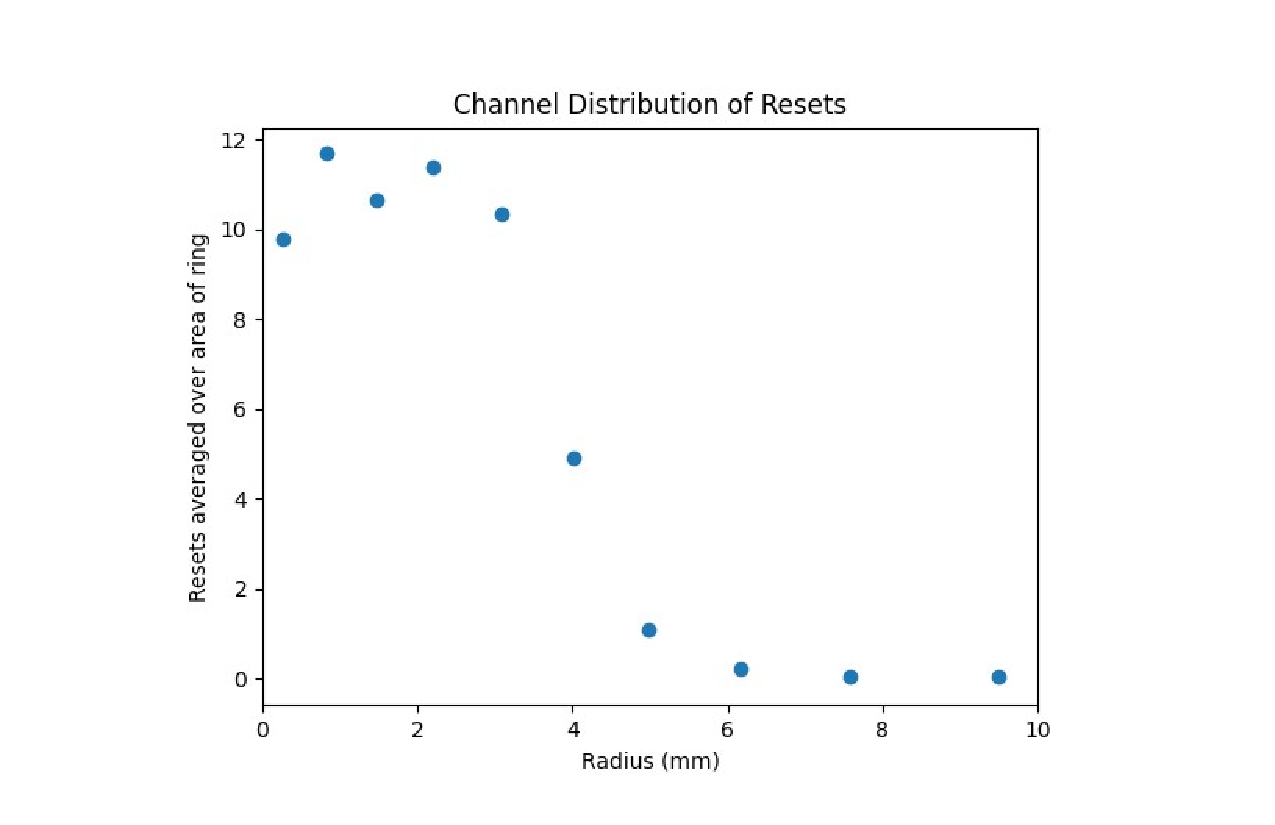
\includegraphics[width=\textwidth]{images/SAQ_first_diffusion_measurement.pdf}
\caption{First diffusion measurement in P-10 gas performed at Wellesy University.}
\label{fig:saq_first_diffusion_measurement}
\end{figure}

\subsection{Planned Measurements}

Measurements of Transverse and Longitudinal diffusion of electrons within electric fields of strength 500 V/cm have been performed before~\citep{lar_diffusion_measurement_LI2016160}.
